% !Mode:: "TeX:UTF-8"
%% 请使用 XeLaTeX 编译本文.
% \documentclass{WHUBachelor}% 选项 forprint: 交付打印时添加, 避免彩色链接字迹打印偏淡. 即使用下一行:
\documentclass[forprint]{WHUBachelor}
\usepackage{geometry}
\usepackage{float}
\usepackage{minted}
\usepackage{algorithm}
\usepackage{algorithmicx}
\usepackage{algpseudocode}
\usepackage{amsmath}

\begin{document}
%%%%%%% 下面的内容, 据实填空.

\title{猴子吃香蕉问题的解决 \\ {\Large《人工智能导论》实验报告}}
\author{马玉坤}                            % 作者名字
\Cmajor{计算机科学与技术}                  % 专业中文名
\Cschoolname{计算机科学与技术系}          % 学院名
\Csupervisor{李钦策}        %指导教师中文名、职称
\date{二〇一八年一月}                    % 日期, 要注意和英文日期一致!!
\teammates{李伟枫,许浩禹,张宁}
\StudentNumber{1150310618}

%-----------------------------------------------------------------------------
\pdfbookmark[0]{封面}{title}         % 封面页加到 pdf 书签
\maketitle
\frontmatter
\pagenumbering{Roman}              % 正文之前的页码用大写罗马字母编号.
%-----------------------------------------------------------------------------
% !Mode:: "TeX:UTF-8"

%%% 此部分需要自行填写: (1) 中文摘要及关键词 (2) 英文摘要及关键词

%%======中文摘要===========================%
\begin{cnabstract}
  在本次CPU设计过程中,本人在两位实验课老师和Digilent社区的帮助下,设计了一个可在Nexys 4 DDR上运行的,有固定指令周期的且支持十条指令的精简指令集 (RISC) 处理器。本文详细介绍了本人在计算机设计与实践实验课上完成计算机设计与实践实验5的相关设计。本文内容包括: (1) CPU的顶层设计; (2) CPU各个模块,包括取指模块、运算模块、访存模块、回写模块、内存控制以及IO控制若干个模块的内部设计; (3)进行CPU设计及实现过程中遇到的问题与解决方法; (4) Digilent Nexys 4 DDR FPGA的简单介绍。

\end{cnabstract}
\par
\vspace*{2em}


%%%%--  关键词 -----------------------------------------%%%%%%%%
%%%%-- 注意: 每个关键词之间用“;”分开,最后一个关键词不打标点符号
\cnkeywords{中央处理器; CPU; FPGA; VHDL; 计算机设计与实践 }
    % 加入摘要, 申明.
%==========================把目录加入到书签==============================%%%%%%
\pdfbookmark[0]{目录}{toc}
\tableofcontents
\mainmatter %% 以下是正文
%%%%%%%%%%%%%%%%%%%%%%%%%%%--------main matter-------%%%%%%%%%%%%%%%%%%%%%%%%%%%%%%%%%%%%

\chapter{简介/问题描述}

\section{解决问题的解释}
查阅资料\cite{AI},编写程序,使用产生式系统、框架系统、语义网络等解决猴子吃香蕉的问题。

\section{问题的形式化描述}

通过给出当前系统的状态与最终状态,计算所需的操作能够使猴子达到最终状态,输出这个操作序列。

\section{解决方案介绍(原理)}

规则库中有五条规则,而综合数据库中只有初始状态。

接下来我们使用程序,对综合数据库中的每个状态,使用规则库中的规则产生新的状态,然后将新状态加入到综合数据库中。重复这一步骤,直到找到目标状态。根据存储的状态转移序列,即可得到所需的操作序列。

\chapter{算法介绍}

\section{所用方法的一般介绍}

我们使用了广度优先搜索算法。使用队列来存储综合数据库中的新状态,直到找到目标状态。

\section{算法伪代码}


\floatname{algorithm}{算法}
\renewcommand{\algorithmicrequire}{\textbf{输入:}}
\renewcommand{\algorithmicensure}{\textbf{输出:}}
\begin{algorithm}[H]
  \caption{通用搜索算法}
  \begin{algorithmic}[1] %每行显示行号
    \Require $initialState$初始状态,$finalState$最终状态
    \Ensure 从初始状态转移到最终状态所需的操作序列
    \State 将开始状态放在综合数据库
    \While {最终状态不在综合数据库中}
    \For {$x \in $综合数据库找到所有没有扩展过的状态}
    \State 对这些状态使用规则库中的五个规则进行状态转移
    \State 将转移得到的状态y加入到综合数据库之中
    \State 并且记录这个状态y的父亲状态是x
    \EndFor
    \EndWhile
    \State 根据最终状态的父亲节点递归寻找,直到找到最初状态,打印状态序列.并且根据状态序列找到猴子的操作序列.
  \end{algorithmic}
\end{algorithm}

\chapter{算法实现}


\section{实验环境与问题规模}

\subsection{实验环境}

\begin{itemize}
\item \textbf{CPU:} Intel E3-1230 V5
\item \textbf{IDE:} Code::Blocks
\item \textbf{操作系统:} Windows 10
\end{itemize}

\subsection{问题规模}

当前系统状态数目是一个五元组,合法的状态数目很少,所以数据规模很小。

\section{数据结构}

在定义状态时,我们使用了五元组来表示($(M, B, Box, On, H)$)。

其中$M$表示猴子的位置 ,$B$表示香蕉的位置, $Box$表示箱子的位置,$On=0$表示猴子在地板上; $On=1$表示猴子在箱子上; $H=0$表示猴子没有抓到香蕉;  $H=1$表示猴子抓到了香蕉。

为了处理方便,我们将状态转化成了一个五位$int$整形数据,我们使用一个长为99999的数组来表示综合数据库,当数组中下标为$i$的元素不是0的时候,表示整数$i$对应的状态在综合数据库之中,同时我们使用$state\_father$数组来记录状态的父亲状态。如果我们使用状态$i$利用规则库之中的规则产生了状态$j$,那么数组中下标为$j$的位置存储的就是$i$。

\section{实验结果}

我们的程序能够根据猴子的最初状态和最终状态找到一个合法的状态转移序列,并且能够根据这个状态转移序列给出猴子每一步需要作出什么操作。

\section{系统中间及最终输出结果}

如图\ref{fig:result}所示,系统最初状态为32200,此时猴子从3移动到了2,状态变为22200。

接着猴子在2上箱子, 状态又变成了22210,最后猴子在2抓到香蕉了,系统到达了最终的状态22211。

\begin{figure}[H]
  \centering
  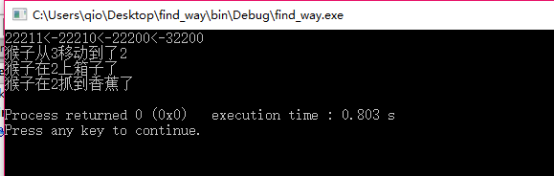
\includegraphics[width=6in]{figures/result.png}
  \caption{结果截图}\label{fig:result}
\end{figure}

\chapter{总结及讨论}

通过本次实验,我们认识到了产生式系统的工作原理,进一步了解了规则库、控制系统和综合数据库的概念。

本次实验中,我与其他组员分工明确,合作无间,完成了本次实验。通过本次实验,我们的友谊得到了升华,对人工智能导论课程内容的理解进一步提高。

%%%=== 参考文献 ========%%%
\cleardoublepage\phantomsection
\addcontentsline{toc}{chapter}{参考文献}
%\bibliographystyle{agsm}
\bibliography{ref}

%%% !Mode:: "TeX:UTF-8"
%%%%%%%%%%%%%%%%%%%%%%%%%%%%-------致谢--------%%%%%%%%%%%%%%%%%%%%%%%%%%%%%%%%

\acknowledgement
\addcontentsline{toc}{chapter}{致谢}

感谢罗丹彦老师和助教学长的耐心指导,实验5的完成离不开他们的指点。











 %%%致谢

%%%-------------- 附录. 不需要可以删除.-----------

\appendix

\chapter{实验代码}
\begin{minted}[fontsize=\small]{C++}

#include <iostream>
#include <string.h>
#include <stdio.h>
using namespace std;
int state_set[99999];//记录综合数据库
int state_father[99999];//记录产生该状态的父亲状态
int state_son[99999];//记录产生正确结果的过程之中,某一个状态的后继状态

int next_state;//记录由状态和规则产生的下一个状态

const int start_state=32200;//用全局变量来表示开始的节点和结束的节点
const int end_state=22211;


int mat[5];
int mat2[5];
void get_value(int i)//将输入的状态i存储到mat数组之中
{
    mat[0]=i/10000;
    mat[1]=(i%10000)/1000;
    mat[2]=(i%1000)/100;
    mat[3]=(i%100)/10;
    mat[4]=(i%10);
}
void get_value2(int i)//将输入的状态存储到mat2数组之中
{
    mat2[0]=i/10000;
    mat2[1]=(i%10000)/1000;
    mat2[2]=(i%1000)/100;
    mat2[3]=(i%100)/10;
    mat2[4]=(i%10);
}


void print(int a,int b)//打印从状态a到状态b需要执行的操作
{
    get_value(a);
    get_value2(b);
    //根据状态a与状态b的区别找到猴子需要执行什么操作
    if(mat[4]!=mat2[4])
    {
       printf("猴子在%d抓到香蕉了\n",mat[0]);
       return;
    }
    if(mat[3]!=mat2[3])
    {
        if(mat2[3]==0)
        {

            printf("猴子在%d下箱子了\n",mat[0]);return;
        }
       if(mat2[3]==1)
        {

             printf("猴子在%d上箱子了\n",mat[0]);return;
        }

    }
    if(mat[2]!=mat2[2])
    {
      printf("猴子从%d把箱子推到了%d\n",mat[2],mat2[2]);return;

    }
     if(mat[0]!=mat2[0])
    {
      printf("猴子从%d移动到了%d\n",mat[0],mat2[0]);return;
    }
}
void addadd(int i)
{
    //printf("next_state=%d\n",next_state);
        if( state_set[next_state]==0)
        {
            state_set[next_state]=1;
            state_father[next_state]=i;
        }
}
int main()
{
    state_set[start_state]=1;//将最初的状态加入到综合数据库
    while(state_set[end_state]==0)//一直循环直到找到最终状态为止
    {
        for(int i=0;i<99999;i++)// 遍历综合数据库中的每一个状态,
                                // 并且用规则库之中的状态产生新的状态
        {
            if(state_set[i]==1)
            {
                next_state=0;
                get_value(i);//将状态进行解码
                //IF (x, y, z, 0, 0) THEN (w, y, z, 0, 0)
                //下面利用规则集合中的第一条规则进行状态扩展,后面的同理
                if(mat[3]==0&&mat[4]==0)
                {
                     next_state=1*10000+i%10000;
                        addadd(i);
                       next_state=2*10000+i%10000;
                      addadd(i);
                       next_state=3*10000+i%10000;
                     addadd(i);
                }
                //IF (x, y, x, 0, 0) THEN (z, y, z, 0, 0)
                 if(mat[3]==0&&mat[4]==0 &&mat[0]==mat[2])
                {
                     Next_state=mat[1]*1000+1*100+1*10000;
                      addadd(i);
                       next_state=mat[1]*1000+2*100+2*10000;
                     addadd(i);
                        next_state=mat[1]*1000+3*100+3*10000;
                      addadd(i);
                }

                //IF (x, y, x, 0, 0) THEN (x, y, x, 1, 0)
                 if(mat[3]==0&&mat[4]==0 &&mat[0]==mat[2])
                {
                     next_state=(i/100)*100+10;
                       addadd(i);

                }
                //IF (x, y, x, 1, 0) THEN (x, y, x, 0, 0)
                 if(mat[3]==1&&mat[4]==0 &&mat[0]==mat[2])
                {
                    next_state=(i/100)*100;
                      addadd(i);
                }
                //: IF (x, x, x, 1, 0) THEN (x, x, x, 1, 1)
                if(mat[0]==mat[1]&&mat[1]==mat[2]&& mat[3]==1&&mat[4]==0)
                {
                    next_state=i+1;
                     addadd(i);
                }
                //当前状态已经扩展完成了,我们使用2来防止以后扩展该状态
                state_set[i]=2;
            }
        }
    }
    //打印状态序列,利用state_father中存储的信息,从终点逆序找到最初开始的节点.
    //在打印正确结果的同时,我们也将信息存储于在state_son之中,方便我们接下来顺序打印操作序列
    printf("%d<-",end_state);
    int father=state_father[end_state];
     state_son[father]=end_state;
    while(father!=start_state){
        printf("%d<-",father);
        state_son[state_father[father]]=father;
        father=state_father[father];
    }
     printf("%d\n",start_state);
    //下面将猴子需要进行的操作逐行打印出来
    int index=start_state;
    while(index!=end_state)
    {
         print(index,state_son[index]);//打印从当前状态到下一个状态需要进行的操作
         index=state_son[index];
    }
    return 0;
}
\end{minted}

\cleardoublepage

\end{document}
